\section{Probabilistic Model}
\label{sec:model}

We have defined unary, binary, and global scoring functions for pattern color properties; we now need a way to combine them all into one unified scoring function that evaluates the overall quality of a pattern coloring.

To do this, we turn to the language of \emph{probabilistic factor graphs}. A factor graph is a type of probabilistic graphical model that decomposes a complex probability distribution over multiple variables into a set of smaller \emph{factors} over smaller subsets of the variables. In our case, the variables $\colorVars$ are the colors of each color group in a pattern, and the factors $\factor$ are derived from the scoring functions defined in the previous sections. Figure~\ref{fig:FactorGraph} shows an example of a factor graph for one simple pattern. The circles denote color variables, while squares denote different factors $\factor$. Edges in the graph connect each factor to the variables within its scope.

\begin{figure}[ht]
%\raisebox{4em}{
\includegraphics[width=.2\columnwidth]{figs/factorGraphPattern}} &
%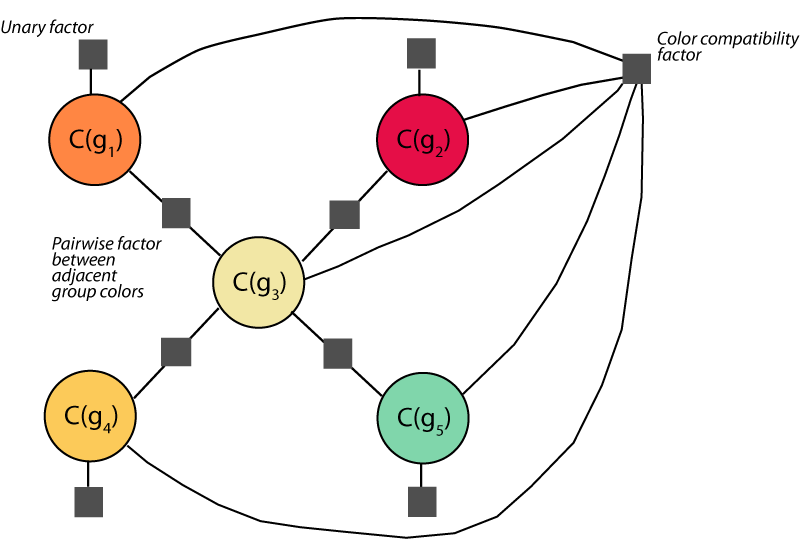
\includegraphics[width=.7\columnwidth]{figs/factorGraph} 
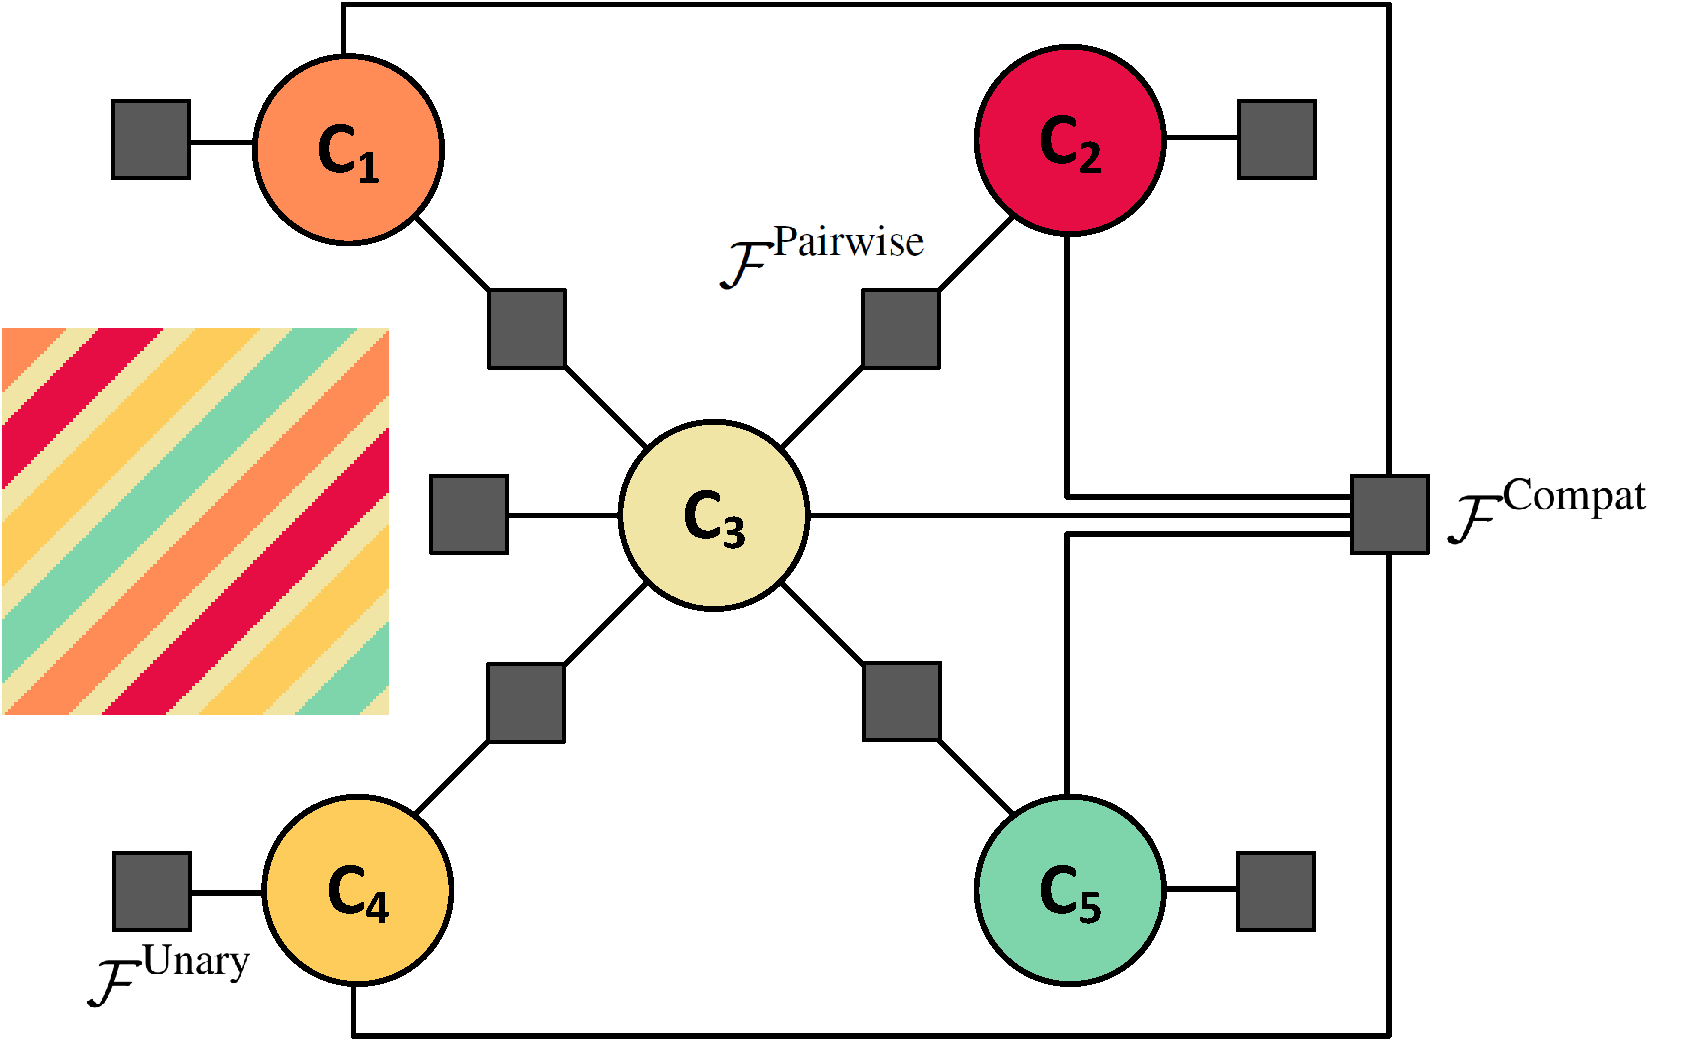
\includegraphics[width=\columnwidth]{figs/factorGraphNew}
\caption{A factor graph for an example pattern template. Variable nodes are colored according to their corresponding color group in the pattern.}
\label{fig:FactorGraph}
\end{figure}

The factors connected to single variables are derived from our unary scoring functions; they combine the score for the color group with the scores for all segments in the group:
%%
\begin{equation*}
 \factor^{\textrm{Unary}}_\prop(\colors_\group) =
 		\exp( \groupTermWeight \cdot \groupInstStats(\colors_\group)  \\
 		     + \segTermWeight \cdot \sum_{\segment \in \group} \segInstStats(\colors_\group)) 
\end{equation*}
%%
The $w$ terms are weights that control the relative importance of each function; we will see how to set them later in this section.

The factors connected to two variables come from our binary scoring functions and combine the scores for all adjacencies which involve segments from two different color groups:
\begin{equation*}
\factor^{\textrm{Binary}}_\prop(\colors_\group, \colors_\groupprime) =
	\exp( \adjTermWeight \cdot \sum_{\mathclap{(\segment, \segprime) \in \adj(\group, \groupprime)}} \adjInstStats( \colors_\group, \colors_\groupprime))
\end{equation*}
%%
Finally, the factor connected to all five color variables enforces color compatibility:
%%
\begin{equation*}
\factor^{\textrm{Compat}}(\colors_1 \ldots \colors_5) = \exp(\colorCompatWeight \cdot \colorCompatInstStats(\colors_1 \ldots \colors_5))
\end{equation*}
%%
The probability distribution encoded by this factor graph is the normalized product of all of these factors:
%%
\begin{equation*}
p(\colors | \pattern : \weights) = \frac{1}{Z(\pattern : \weights)} \prod_{\factor} \factor(\textit{Scope}_\factor(\colors))
\end{equation*}
%%
Here, $\textit{Scope}_\factor$ selects the color variables connected to the factor $\factor$ and $Z(\pattern : \weights)$ is the pattern-dependent partition function that normalizes the distribution. The distribution is parameterized by the vector of factor weights $\weights$.

%We formulate the problem of generating colorings for a pattern template as finding high-probability colorings under a probabilistic model.
%
%We define the probability of a coloring for a particular pattern template as a log-linear model:  
%\begin{equation*}
% p(\colors | \pattern : \weights) = \frac{1}{Z_\pattern(\weights)} \prod_{\term \in \model} \exp(\termWeight \cdot \termStats(\colors, \pattern))
%\end{equation*}
%The model $\model$ is comprised of a number of different terms $\term$, where each term scores the goodness of a color assignment based on a term-dependent statistic $\termStats(\colors,\pattern)$. $Z_\pattern(\weights)$ is the pattern-dependent partition function that normalizes the distribution. Each term also has a weight $\termWeight$ which determines its relative contribution to the model; the method used for setting these weights is detailed in Section~\ref{sec:weights}. Bolded symbols are vector-valued while non-bolded symbols are scalar.
%
%This type of model is well-suited to the coloring-generation problem. It is very flexible; in principle, the individual term statistics $\termStats$ can be any real-valued function. In our model, we include terms both for color compatibility as well as for spatial properties defined over groups, segments, and segment adjacencies. Users can also guide the model via additional soft constraint terms (Section~\ref{sec:results}). In addition, it is very easy to compare the relative importance of each term by comparing their weights, which we will do in Section~\ref{sec:weights} to gain some insight into which terms contribute the most to producing attractive colorings. 
%
%The model can also be interpreted graphically as a factor graph (Yeh et al.~\shortcite{YiTingTiledPatterns} provides an accessible introduction for the graphics community). Each type of term contributes different factors $\factor$ to the graph. For example, our color compatibility term contributes a factor over at most five color variables that scores the compatibility of those colors. The spatial terms contribute a unary factor for each color variable and binary factors for color variables that are adjacent in the pattern. Figure~\ref{fig:FactorGraph} shows an example of such a factor graph. Circles denote the color variables, while squares denote the different factors $\factor$, and edges connect each factor to the variables within their scope. 
%
%
%\begin{figure}[ht]
%\begin{tabular}{cc}
%\raisebox{4em}{
\includegraphics[width=.2\columnwidth]{figs/factorGraphPattern}} &
%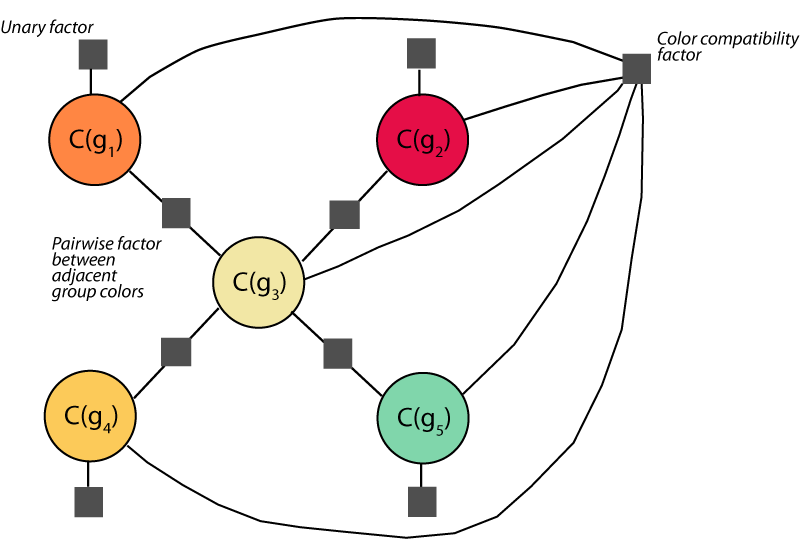
\includegraphics[width=.7\columnwidth]{figs/factorGraph} \\
%\end{tabular} 
%\caption{A factor graph for an example pattern template. Factors correspond with the color compatibility and spatial terms from our model. In the figure, nodes are colored according to their corresponding color group in the pattern\remark{Rough figure.}}
%\label{fig:FactorGraph}
%\end{figure}


\subsection{Sampling}
\label{sec:sampling}

To generate good coloring suggestions, we must sample high-probability states from the model. We use the Metropolis-Hastings algorithm (MH), a variant of Markov Chain Monte Carlo (MCMC), to sample coloring suggestions~\cite{Metropolis,Hastings}. MH explores the coloring state space by \emph{proposing} candidate new states; these proposals are accepted with probability proportional to their model score. We would also like our sampler to output a variety of different suggestions, which requires that it explore many modes of the distribution. To do this efficiently, we employ parallel tempering, a technique that runs multiple MCMC chains in parallel at different `temperatures' and swaps their states periodically~\cite{ParallelTempering}. `Hot' chains are more likely to take large jumps across the space of possible colorings, whereas `cool' chains behave like local hill-climbing optimizers. The combined system of chains effectively explores and refines different coloring configurations.

Our sampler uses the following MH proposals:
\begin{itemize}
	\item{\textbf{Perturb} a randomly chosen color by $v \sim \mathcal{N}(0, \sigma)$ in RGB space}
	\item{\textbf{Swap} two randomly chosen colors}
\end{itemize}
where $\sigma$ varies linearly with the model temperature $t$, encouraging larger perturbations at high temperatures. The sampler chooses between these two proposals with probability $\rho$, which also varies linearly with temperature. The sampler operates in RGB space since all RGB colors fall in the gamut of human color vision, which is not the case with \lab space. Since the RGB color space is bounded, the perturbation proposal draws from a truncated normal distribution in order to maintain ergodicity of the MCMC chains~\cite{TruncatedGaussians}.

%Rather than sample directly from the distribution encoded by the model, we sample from an \emph{annealed} distribution of the form $p(\colors | \pattern : \weights)^\frac{1}{t}$, where $t$ is a `temperature' term that controls the peakiness of the distribution.
%We use the Metropolis-Hastings algorithm (MH), a variant of Markov Chain Monte Carlo (MCMC), to sample coloring suggestions~\cite{Metropolis,Hastings}. MH explores the coloring state space by \emph{proposing} candidate new states; these proposals are accepted with probability proportional to their model score. Our sampler uses the following proposals:
%\begin{itemize}
%	\item{\textbf{Perturb} a randomly chosen color by $v \sim \mathcal{N}(0, \sigma)$ in RGB color space}
%	\item{\textbf{Swap} two randomly chosen colors}
%\end{itemize}
%where $\sigma$ varies linearly with the model temperature $t$. The sampler chooses between these two proposals with probability $\rho$, which also varies linearly with temperature. Since the RGB color space is bounded, the perturbation proposal draws from a truncated normal distribution in order to maintain ergodicity of the chain~\cite{TruncatedGaussians}.
%
%Asymptotically, MCMC samples states with a frequency proportional to their probability under the model. In practice, it can take a prohibitively long time to explore all the modes of a distribution as complex as the one encoded by our model. We would like our sampler to explore as many modes as possible so that it can suggest multiple, high-probability coloring states.
%
%To accelerate sampling, we use parallel tempering, a technique that runs multiple MCMC chains in parallel at different temperatures and swaps their states periodically~\cite{ParallelTempering}. Large values of $t$ yield flatter probability landscapes, so these `hot' chains are more likely to take large jumps across the state space. `Cool' chains, on the other hand, reject almost all proposed states that do not lead to higher probabilities, thus behaving like local hill-climbing optimizers. Running multiple chains in parallel allows the total system to alternatively explore and refine different coloring configurations.

Finally, we use maximimum marginal relevance (MMR) to enforce diversity in the set of suggestions returned by the sampler~\cite{MMR}. MMR is a technique from information retrieval that re-ranks every item in a list according to a linear combination of relevance (model score, in our case) and similarity to the items preceding it. The similarity metric we use for two colorings $\colors$ and $\tilde{\colors}$ of a pattern is $- \sum_{\group \in \groups} {\size_\group \cdot ||\colors_\group - \tilde{\colors}_\group||}$, which is the area-weighted sum of \lab distances between the corresponding colors in each coloring.

\subsection{Weight Learning}
\label{sec:weights}

The factor graph model we have defined is parameterized by a vector of weights $\weights$. Setting these weights manually proves challenging, as it is not obvious which color properties matter most to the quality of a pattern coloring. Instead, we would like to set them automatically, using our training dataset as a guide.

We formualate the weight-tuning problem as one of \emph{maximum likelihood parameter estimation}. That is, we would like to set the weights such that the training examples have high probability under the resulting model. We first rewrite the probability distribution encoded by our model from a weight-centric view
%%
\begin{equation*}
p(\colors | \pattern : \weights) = \frac{1}{Z(\pattern : \weights)} \prod_{w \in \weights} \exp(w \cdot \weightStats(\colors, \pattern))
\end{equation*}
%%
where $\weightStats(\colors, \pattern)$ simply sums all the scoring functions $\phi$ that share the weight $w$. We can then easily express the log-likelihood of the the weights given a dataset $\dataset$ of pattern colorings:
%%
\begin{equation*}
\ell(\weights : \dataset) =
	\sum_{(\pattern, \colors) \in \dataset}
	(
		\sum_{w \in \weights}
			w \cdot \weightStats(\colors, \pattern)
	)			
		- \ln{Z(\pattern : \weights)}
\end{equation*}
%%
Convex log-likelihoods such as this one are typically maximized via gradient ascent. The partial derivatives of this function with respect to the weights are
%% Partial derivatives
\begin{equation*}
\frac{\partial}{\partial w} \ell(\weights : \dataset) = 
	\sum_{(\pattern, \colors) \in \dataset}
			\weightStats(\colors, \pattern)
		- \expectation_\weights[\weightStats(\colorVars, \pattern)]
\end{equation*}
%%
where $\expectation_\weights$ denotes an expectation under the model with weights $\weights$. Unfortunately, these quantities are extremely expensive to compute. The expectation term requires probabilistic inference---an NP-complete problem---for every training pattern, for every iteration of gradient ascent.

This computational intractability has motivated the development of alternative, `biased' parameter estimation schemes which do not directly maximize the likelihood function but nevertheless yield parameters that give high likelihoods. We use one such method, called \emph{Contrastive Divergence} (CD)~\cite{ContrastiveDivergence}. CD uses the following approximation to the likelihood gradient:
%% CD gradient
\begin{equation*}
CD^k_w(\weights : \dataset) = 
	\sum_{(\pattern, \colors) \in \dataset}
			\weightStats(\colors, \pattern)
		 -\weightStats(\hat{\colors}, \pattern)
\end{equation*}
%%
where $\hat{\colors}$ is the coloring state obtained by running an MCMC chain for $k$ steps from the initial state $\colors$. CD essentially forms a local approximation to the likelihood gradient around the neighborhood of state $\colors$. Larger $k$ yields more accurate approximations at additional cost; we use $k = 10$ in our experiments. We initialize the weights uniformly to 1 and constrain them to be non-negative, since all terms in the model are log-probabilities.

While the exact weights learned depend on the training dataset, there are several persistent trends.
The perceptual difference, color compatibility, and color name count terms receive the highest weights. These trends coincide well with our intuition that colors should be harmonious, adjacent regions should have sufficient contrast, and colors should be categorically similar to those in the training set.
The lowest weight belongs to the color name similarity term, which suggests that the similarity in how two colors are named is not strongly predictive of their compatibility as an adjacent color pair.
%The information conveyed by this property may be partially redundant with the perceptual difference term. Also, as this property computes the cosine similarity between two 179-dimensional color name count vectors, the dimensionality of the color name space may simply be too high to provide sufficient discrimination for pattern coloring.

\subsection{Implementation}
\label{sec:implementation}

Our prototype implementation of this model is written in the Scala programming language, using the Factorie toolkit for probabilistic modeling~\cite{Factorie}. To evaluate the color compatibility term, it uses the reference MATLAB implementation provided by O'Donovan et al.~\shortcite{ODonovan}. A link to the source code can be found on the project website.